\chapter{Seismic Noise}
Seismic noise limits the low-frequency sensitivity of gravitational-wave detectors and degrades the duty cycle of that. In this chapter,以下の事柄を述べる;
\begin{itemize}
\item 地面振動の数学的な理解とその性質(\cref{sec:31})
\item 一般的な地面振動のノイズ源(\cref{sec:32})
\item KAGRAの地面振動の時間的な特徴(\cref{sec:33})
\item KAGRAの地面振動の空間的な特徴(\cref{sec:34})
\end{itemize}


\section{Theory of seismic waves} \label{sec:31}
Here we introduce characteristics of the seismic wave that will be usefull in our later understanding and modeling of seismic effects.

\subsection{Seismic Waves in Isotropic and Homogeneous Medium}
The elastrodynamic wave equation is given by 
\begin{eqnarray}\label{eq:eq_1}
  \rho{\bm{\ddot{u}}} = (\lambda+2\mu)\nabla(\nabla\cdot\bm{u}) - \mu\nabla\times(\nabla\times\bm{u}),
\end{eqnarray}
where $\bm{u}$ is the displacement field vetor of the medium, $\rho$ denotes density of the medium, and $\lambda,\,\mu$ are Lame's first and second constant.

\subsubsection{Body Waves}
From \ref{eq:eq_1}, we can obtain two characteristic waves; primary wave (P-wave) which is a longitudinal wave and secondary wave (S-wave) which is a transverse wave. Using Helmholtz's decomposition, we represent the displacement field vector $\bm{u}$ as
\begin{eqnarray} 
  \bm{u} &=& \nabla\phi + \nabla\times\bm{\psi}, \label{eq:eq_4}
\end{eqnarray}
where $\phi$ the scalar potential and $\bm{\psi}$ are the vector potential. Each term of \ref{eq:eq_4} show the divergent and the rotation component of $\bm{u}$ respectively. Substitute Eq. \ref{eq:eq_4} into Eq. \ref{eq:eq_1} and after some vector algebra, one can obtain two wave equations;
\begin{eqnarray}
  \ddot{\phi} &=& v_{L}^2\nabla^2\phi \label{eq:eq_5},\\
  \ddot{\psi} &=& v_{T}^2\nabla^2\psi \label{eq:eq_6}, 
\end{eqnarray}
where $v_{L},\,v_{T}$ are defined as 
\begin{eqnarray}
  v_{L} = \sqrt{\frac{\lambda+2\mu}{\rho}},\
  v_{T} = \sqrt{\frac{\mu}{\rho}}. \label{eq:eq_7}
\end{eqnarray} 
These phase velocities; $v_{L},v_{T}$ represent that of the P-wave and the S-wave. Show this relationships. Because the scalar potential and the vector potential are obey the wave equation Eq.\ref{eq:eq_5} and Eq.\ref{eq:eq_6} respectivly, the general solutions of these potentials are given as
\begin{eqnarray}
  \phi &=& \phi_{0}(\omega{t}-\bm{k}\cdot{\bm{x}}) \label{eq:eq_8}\\
  \bm{\psi} &=& \bm{\psi_{0}}(\omega{t}-\bm{k}\cdot{\bm{x}}) \label{eq:eq_9},
\end{eqnarray}
where $\omega,\,\bm{k}$ are the angler frequency and the wave vector. One can obtain the divergent component of displacement filed vector $\bm{u}$ as
\begin{eqnarray}
  \bm{u}_{\mathrm{div}} = \nabla{\phi_{0}(\omega{t}-\bm{k}\cdot{\bm{x}})} =-\bm{k}{\phi}.
\end{eqnarray}
The displacement of this wave $\bm{u}_{\mathrm{div}}$ whose phase velocity is $v_{L}$ propagates along with direction of the wave vector. Therefore $v_{L}$ is the phase velocity of a longitudinal wave called P-wave. On the other hands, one can obtain the rotation component of $\bm{u}$ as
\begin{eqnarray}
  \bm{u}_{\mathrm{rot}} = \nabla\times{\bm{\psi_{0}}(\omega{t}-\bm{k}\cdot{\bm{x}})} =-\bm{k}\times{\bm{\psi}}.
\end{eqnarray}
This displacement vector $\bm{u}_{\mathrm{rot}}$ whose phase velocity is $v_{T}$ is perpendicular to the wave vector. Therefore, $v_{T}$ is the phase velocity of a transverse wave called S-wave. Furthermore, because  $\lambda$ and $\mu$ are positive numbers, 
\begin{eqnarray}
  v_{L} > v_{T}.\label{eq:eq_10}
\end{eqnarray}
Therefore, the longituginal wave is faster than the transverse wave.

\subsubsection{Rayleigh waves}
Rayleigh wave はP波とS波の干渉によって生じる\cite{}。ここではZ軸を鉛直方向とした直交直線座標系のx-z面内で振動する弾性波を考える。z=0を自由表面とし、x軸に沿ってP波とS波が同じ速度$v_{R}=\omega/k$ ($\omega$ is anglar frequency and $k$ is the wave vector) で伝搬する場合を考えると、ポテンシャル$\phi$と$\bm{\psi}$は、それぞれ以下のように表すことができる。
\begin{eqnarray}
  \phi &=& F(z)\exp[i(kx-\omega{t})],\label{eq:eq_12}\\
  \psi &=& G(z)\exp[i(kx-\omega{t})]\label{eq:eq_13}
\end{eqnarray}
Eq.\ref{eq:eq_12}とEq.\ref{eq:eq_12}を波動方程式Eq.\ref{eq:eq_5},Eq.\ref{eq:eq_6}に代入すれば、レイリー波の特性方程式が導かれる;
\begin{eqnarray}\label{eq:eq_11}
\left(\frac{c_{R}^{2}}{c_{S}^{2}}\right)^{3}-8\left(\frac{c_{R}^{2}}{c_{S}^{2}}\right)^{2}+8\left(3-\frac{2}{\gamma^2}\right)\left(\frac{c_{R}^{2}}{c_{S}^{2}}\right)-16\left(1-\frac{1}{\gamma^2}\right)=0
\end{eqnarray}
where $\gamma\equiv v_{L}/v_{T}$. In case that $0 < (\frac{c_{R}^2}{c_{S}^2}) <1$, the velocity has physically meaningful value. According to Eq.\ref{eq:eq_11}, the ratio $\frac{c_R}{c_S}$ is a function of the ratio of $\gamma$. たとえば、KAGRAと同じ山の下に建設された100mの重力波望遠鏡CLIOでのP波とS波の位相速度はそれぞれAA、BBである\cite{takemoto2003}ので、$\gamma = 1.82 $である。したがってこのときのレイリー波の位相速度はCCである。


\subsection{Reduction Effect in the Deep Sites}
レイリー波の振幅は深さに依存しており、深いほど小さくなる。



\subsection{Reduction Effect of the Short Baseline}
For interferometric gravitational-wave detectors which need a precise length control of the optical resonate cavity, it is appropriate to consider about the relative displacement between two points rather than the displacement of single point. In this subsection, the reduction effect of relative displacement if the seismic noise at each point have a correlation is discribed.

\subsubsection{Differential Motion and Common Motion}
\begin{figure}[h]
  \begin{center}
    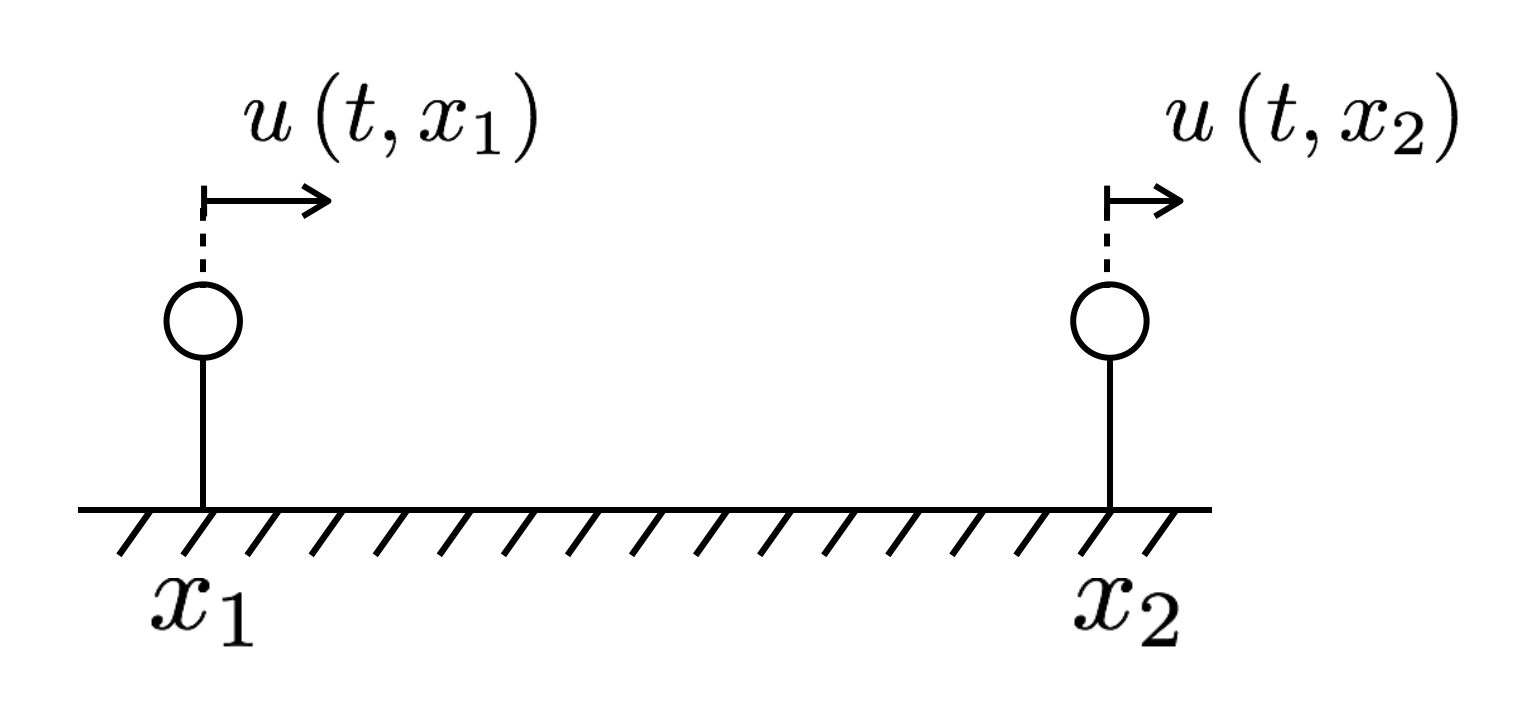
\includegraphics[width=10.0cm]{./img_chap3/img315.png}
    \caption{The displacements of the two points which are sparated L in X axis. }
  \end{center}
\end{figure}

Motions of the two points can be represented as the differential motion and the common motion. Displacement of both differential motion and common motion of the two points shown in Figure(\ref{img:img_chap310}) are defined as
\begin{eqnarray}\label{eq:eq22}
  u_{\mathrm{diff}} \equiv \frac{u_{1}-u_{2}}{\sqrt{2}}, \,
  u_{\mathrm{comm}}  \equiv \frac{u_{1}+u_{2}}{\sqrt{2}}
\end{eqnarray}
where $u_{1}(x,t)$ and $u_2(x,t)$ are the displacement of each points. These two motions defined in Eq.(\ref{eq:eq22}) are normalized by $\sqrt{2}$ due to conserve the total power.


\subsubsection{Common and Differential Motion Ratio (CDMR)}
CDMR is defined as the powers of common motion over the differential motion as bellow,
\begin{equation}
  \mathrm{CDMR} \equiv \sqrt{\frac{\mathrm{Common\,Motion}}{\mathrm{Differential\,Motion}}} = \sqrt{\frac{P_{\mathrm{comm}}(\omega)}{P_{\mathrm{diff}}(\omega)}} \label{eq:eq23}
\end{equation}
where $P_{\mathrm{comm}},P_{\mathrm{diff}}$ are the power spectral densities (PSDs) of the differential motion and common motion, respectively. Each PSDs are converted from the autocorrelation function of these by the Wiener-Khinchin theorem.

First, autocorrelation function $C_{\mathrm{diff}}$ of the differential motion is given by its definition in Eq.(\ref{eq:eq22})
\begin{eqnarray}
  C_{\mathrm{diff}}(\tau) &=& \frac{1}{2}
  \biggl\langle
  \biggl[ x_{1}(t)-x_{2}(t) \biggr] \biggl[ x_{1}(t+\tau)-x_{2}(t+\tau) \biggr]
  \biggr\rangle \\
  &=& \frac{1}{2}\biggl[ C_{11}(\tau) - C_{12}(\tau) - C_{21}(\tau) + C_{22}(\tau) \biggr], 
\end{eqnarray}
,where $C_{ij}$ are the autocorrelation functions of each point and defined as $ C_{ij} \equiv \langle x_{i}(t)x_{j}(t+\tau)\rangle,\, (i=1,2,\,j=1,2)$. Therefore, the power spectrum density of differential motion $P_{\mathrm{diff}}(\omega)$ can be computed as
\begin{eqnarray}
  P_{\mathrm{diff}}(\omega) &=& \frac{1}{2}\biggl[ P_{1}(\omega) + P_{2}(\omega) - P_{12}(\omega) - P_{12}^*(\omega) \biggr]\\
  &=& \frac{1}{2} \biggl[ P_{1}+P_{2} - \mathrm{Re}\left[\gamma \right]\times2\sqrt{P_{1}P_{2}} \biggr] \label{eq:eq31}
\end{eqnarray}
where $P_{1}(\omega),P_{2}(\omega)$ are the power spectrum densities of each points, and $P_{12}(\omega)$ are the cross spectrum between two point. The parameter $\gamma$ is the complex coherence between them defined below,
\begin{eqnarray}
  \gamma \equiv \frac{P_{12}}{\sqrt{P_{1}P_{2}}}.
\end{eqnarray}

Here, assuming that seismic wave propagating each points does not decay, which means $P_{1}=P_{2} \equiv P$, one can compute the $P_{\mathrm{diff}}(\omega)$ as 
\begin{eqnarray}
  P_{\mathrm{diff}}(\omega) = P (1-\mathrm{Re}\left[\gamma\right]).
\end{eqnarray}
Therefore, the PSDs of the common motion can be calculated as
\begin{eqnarray}
  P_{\mathrm{comm}}(\omega) = P (1+\mathrm{Re}\left[\gamma\right]).
\end{eqnarray}
Finaly, CDMR defined Eq.(\ref{eq:eq23}) in case the seismic wave does not decay is represented as
\begin{eqnarray}
 \mathrm{CDMR} = \sqrt{\frac{1 + \mathrm{Re} \left[\gamma \right] }{1 - \mathrm{Re} \left[\gamma \right]}}\,. \label{eq:eq33}
\end{eqnarray}
Eq.(\ref{eq:eq33}) indicate that CDMR can be expressed by only the coherence $\gamma$ between of two points. For example, CDMR tends to be larger when $\gamma$ close to 1. This means that the differential motion is more less than the common motion because the two points move together in the same direction.


\section{Seismic Noise}\label{sec:32}
Characteristics of seismic noise are related with its origin spatially and temporally. The noise sources are spreaded anywhere; foot steps, traffics and ocean waves, and these amplitude depends on day-night or weather condition.

As summarized in Table \ref{tb:31}, the seismic noises above $1\,\mathrm{Hz}$ are cleary correlated with cultural activities, and that below this frequency are excited by the natural phenomena \cite{bonnefoy2006nature}. This boundary frequency between cultural or natural, $1\,\mathrm{Hz}$, is depends on the soil structure. At the sediment site such as the LIGO\cite{Daw_2004} and Virgo site\cite{Beker_2012}, the former noise can be shifted to a lower frequency and appear below $1\,\mathrm{Hz}$. On the other hands, at the hard rock site such as KAGRA site, the cultural noise can be distinguished from the natural noise for its diurnal variability and apparent only above $1\,\mathrm{Hz}$.

\begin{table}[h] 
  \begin{center}
    \caption{Two types of seismic noise}\label{tb:31}
    \begin{tabular}{lll} 
      \hline      
      Type of noise & Frequency Band & Sources \\ \hline \hline
      Cultural Noise & $> 1\,\mathrm{Hz}$ & wind, traffic, machinaries, foot steps\\
      Natural Noise  & $< 1\,\mathrm{Hz}$ & ocean, air pressure, earth tides\\
    \end{tabular}
  \end{center}
\end{table}

\subsection{Cultural Noises} \label{sec:321}
The cultural seismic noise contaminates the sensitivity of gravitational-wave detectors in the frequency range of interest for gravitational-waves sources, above $1\,\mathrm{Hz}$. In this frequency band, the cultural noise is dominated by winds or human activities. For example, seismic noise from traffic near the detectors is reported at LIGO site \cite{schofield2000source}, and noise from the vibrations of building excited by winds is reported at Virgo site \cite{acernese2004properties}. 

\subsection{Natural Noises} \label{sec:322}
The natural seismic noise affects the stability of the GW detectors below $1\,\mathrm{Hz}$ because it deforms largely the bedrock on which mounted the detectors. これらnatural seismic noise は低周波になればなるほどグローバルな励起源によるノイズを反映しており、パワースペクトル密度は大きくなる。

\subsubsection{Microseisms}
Microseisms which power spectrum has peaks in $50$--$200\,\mathrm{mHz}$ are excitated by oceanic waves. These seismic waves can be categolized by the generating mechanism of these \cite{Bormann2012new}. First, the primary ocean microseisms are generated only in shallow waters in coastal regions. In this regions, the water wave enery can be converted directly into seismic energy either through vertical water pressure variations, or by the impacts of surf on the shores. There are correlation between this microseismic peak and the swell at the beaches was known starting from the data sets studied by \cite{haubrich1963comparative}. Second, the secondary ocean microseisms could be explained by the superposition of ocean waves of equal period traveling in opposite directions. Therefore, generating standing gravity waves of half the period \cite{longuet1950theory}.

The RMS amplitude spectral of both type of the microseisms are strongly depends on the low pressure on the ocean \cite{naticchioni2014microseismic}.

\begin{figure}[p]
  \begin{center}
    \begin{minipage}{0.65\hsize}
      \centering
      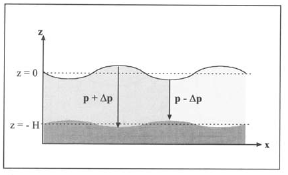
\includegraphics[width=9.0cm]{./img_chap3/img311.png}
      \subcaption{Generating mechanism of the primary microseisms.引用先の図をコピペしているので、自分で描いたのに差し替える。}\label{img:img311}
    \end{minipage}
    \begin{minipage}{0.65\hsize}
      \centering      
      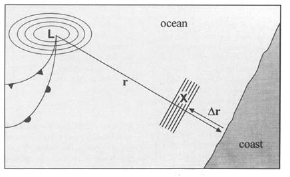
\includegraphics[width=9.0cm]{./img_chap3/img312.png}
      \subcaption{Generating mechanism of the secondary microseisms.引用先の図をコピペしているので、自分で描いたのに差し替える}\label{img:img312}
    \end{minipage}
  \end{center}
  \caption{ Generating mechanism of the microsisms. \subref{img:img311} describes the mechanism of the primary microseisms. \subref{img:img312} describes the mechanism of the secondary microseisms.}
\end{figure}

\subsubsection{Deformation of the bedrock}
In few mHz, ground defromed by the air pressure changes. 
...\\
...\\

Below more lower frequency, the earth deformed by tidal forces due to the attraction of the Sun and the Moon. 

\subsection{Spatial Seismic Noise Changes}
地面振動は場所や時間により異なる。Petersonらは、世界の75箇所の基地にある地震計の数年分のデータから地面振動のノイズスペクトルを得た。これらデータは地表と地下両方のデータを含み、並進成分と垂直成分を含む。NHNMは、内陸の沖積層で地面が揺れやすい場所や、沿岸地域で脈動や人間の活動の影響を受けやすい場所の地面振動を反映している。一方でNHNMは、とくに0.1Hz以下では、広範囲の複数の地震計の垂直成分で得られた地面振動のノイズフロアである。


\begin{figure}[h]
  \begin{center}   
    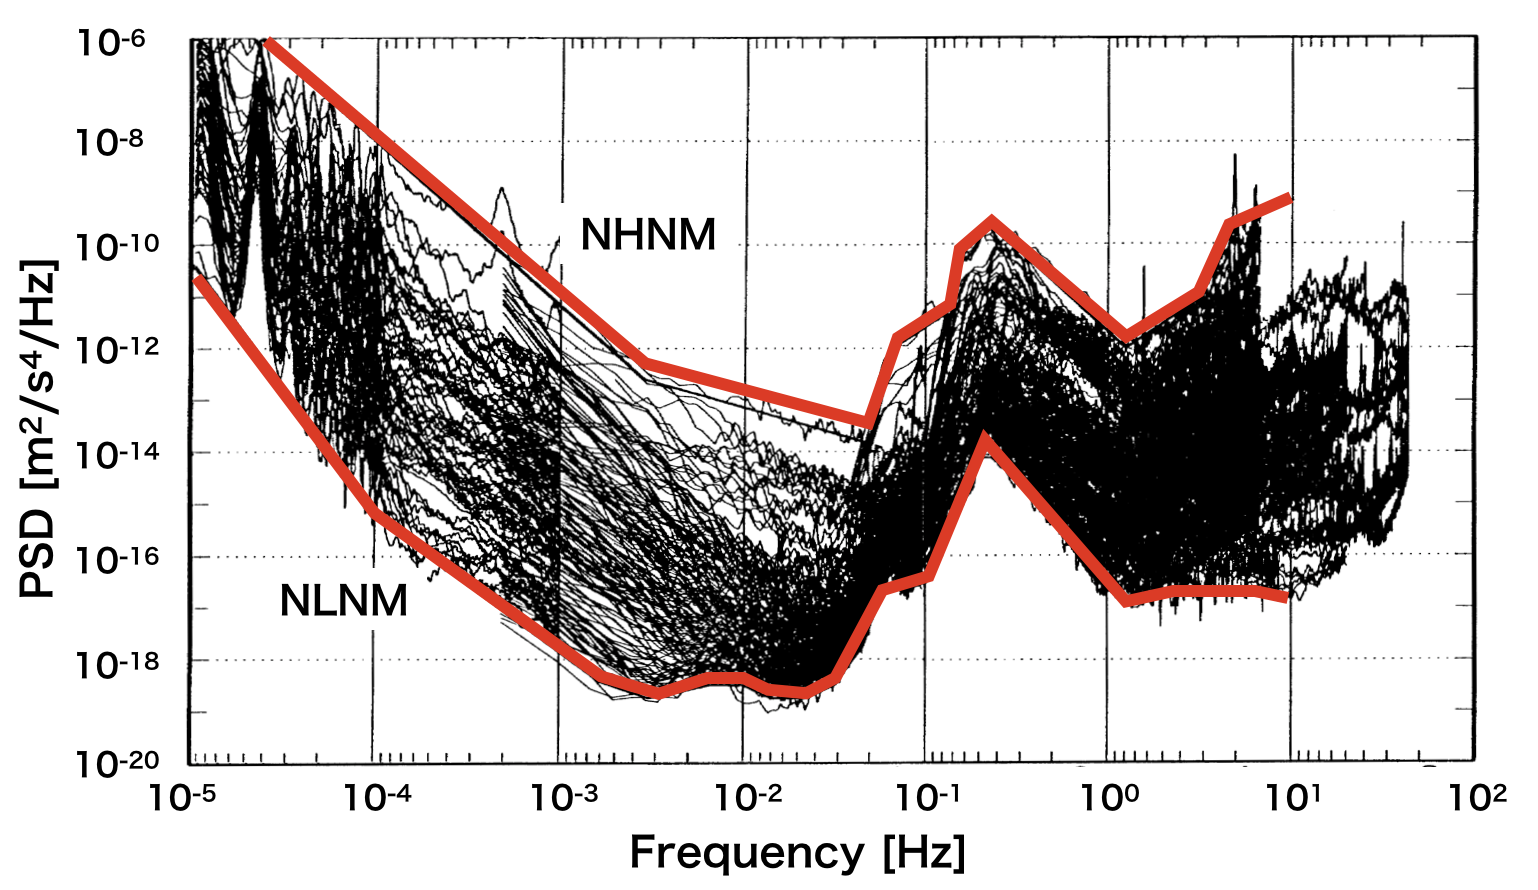
\includegraphics[width=12.5cm]{./img_chap3/img324.png}
    \caption{PSD of the seismic noise obtained by Peterson in several place in the world\cite{peterson1993observations} (この図は自分で書き直す必要あり。)}\label{img:img324}
  \end{center}
\end{figure}


%\newpage
\section{Study of Temporal Seismic Noise at KAGRA} \label{sec:33}
\subsection{Overview}
本節では、KAGRAでの地面振動の大きさが時間帯や季節の違いでどのように変化するか調べた。基本的に地震などの突発現象を除けば、地面振動は定常的な振る舞いを示すが、そのRMS振幅は時間依存である。例えば、人間由来の地面振動は夜間になると静かで、波浪由来の脈動は天気が悪化するとうるさくなる。また日本の場合、初秋は台風によって、冬は日本海低気圧によって脈動がうるさくなることが知られている\cite{}。とくに後者の脈動がうるさいと、干渉計の稼働が妨げられ、DutyCycleを低下してしまう。このような理由から、地面振動の時間依存性を知ることは、干渉計の稼働の安定性を議論するうえで重要である。


地面振動の振幅スペクトルの分布は、およそ1年間の地震計の時系列データからもとめた。このデータには、地震計のメンテナンスによるデータの欠損や、地震などの突発的な地面振動のデータが含まれている。そのため、スペクトルを計算するためにこれらデータを取り除き、およそ1時間(4096秒)区切りのデータ・セットを用意した。これらデータ・セットごとに振幅スペクトルを計算し、分布をもとめた。

\subsection{Experimental Arrangement}
Seismic motion is measured by a seismometer installed on the second floor of the X-end area. This area is placed 200 $\mathrm{m}$ underground from the surface of the mountain. Comparison to corner area, human activity in the end area is less because the corner area has parking lots. Comparison to the Y-end area, there is no entrance connected to other mines. Therefore, the X-end area is relatively quiet in the KAGRA mine, regarding the seismic noise induced by human activity.

In this study, Trillium 120-QA which is known as three-component, very broadband, and low-noise seismometer, was used. These three outputs are proportional to the ground velocity of two horizontal and one vertical, respectively. The feature of the low-noise can resolve  Peterson's new low-noise model (NLNM) and new high-noise model (NHNM) \cite{peterson1993observations}.

\begin{figure}[h]
  \begin{center}   
    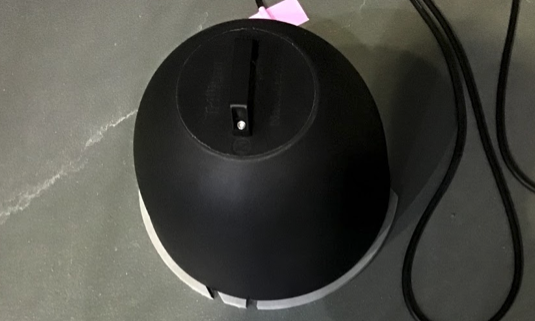
\includegraphics[width=9.0cm]{./img_chap3/img316.png}
    \caption{Trillium 120-QA installed on the second floor at X-end area, which is coverd by black thermal insulation cover}\label{img:img316}
  \end{center}
\end{figure}

As shown in fig \ref{img:img316}, the seismometer is housed in the black thermal insulation cover according to the installation manual \cite{trillium120manual}. Thermal insulation protects two broad categories of thermal couplings that can cause unwanted noise \cite{trillium120manual}. First is the direct coupling to the sensitivity. This coupling typically increases the noise of the vertical channel as a periodic diurnal variation caused by the day-to-night temperature cycle, because the springs that suspended the inertial masses are temperature sensitive. The second is the coupling to tilt from the thermal fluctuation. Tilt converts the vertical acceleration of gravity into horizontal acceleration. This thermally induced tilt noise on the horizontal will be larger than the direct thermal coupling on the vertical channel. To be low sensitivity to both tilt and temperature, this model has a function to center the inertial mass after the initial installation.

The signals of the seismometer is recorded through the data aquisition system developed by LIGO \cite{bork2001overview}. The analog signal is converted to digital signal by the 16 bit analog-to-digital converters (ADC) with 16384 $\mathrm{Hz}$ sampling. This analog signal is amplified with 30 db so that the ADC noise does not mask this signal. 



\subsection{Data Selection}
およそ1年分の地震計のデータをつかった。スペクトルの計算のために、一年分のデータを4096秒のセグメントに分割し、その中からデータの欠損などの異常値を取り除いた。解析に使ったセグメントをFig\ref{img:img317}に示す。14-15週と33-34週に生じた大きなデータの欠損期間を除いて、一年を通してデータが取得できている。セグメントはXX個あり、全体のXX\%を占める。

%% \begin{figure}[H]
%%   \begin{minipage}[b]{0.65\hsize}
%%     %\centering    
%%     
\includegraphics[width=18.0cm]{./img_chap3/img317.png}
%%     \subcaption{各状態の時間分布。}\label{img:img317_a}
%%   \end{minipage}
%%   \begin{minipage}[b]{0.65\hsize}
%%     \centering              
%%     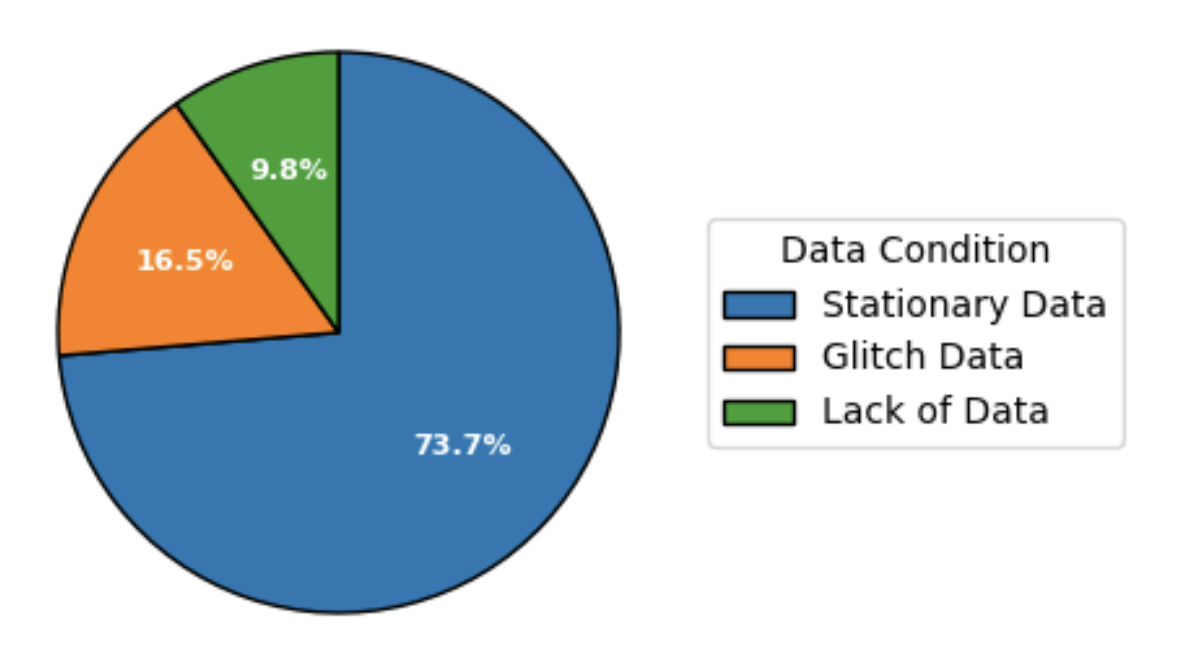
\includegraphics[width=13.0cm]{./img_chap3/img323.png}
%%     \subcaption{各状態の割合。\subref{img:img317_a}を円グラフにしたもの。}\label{img:img317_b}
%%   \end{minipage}
%%   \caption{Available data from June 01 2018 to 2019-06-24 09:40:14JST. Total:全体のセグメント。Lack of Data:データの欠損が合ったセグメント。Glitch:Glitchがあったセグメント。Available:欠損もGlitchもなかったセグメント}\label{img:img317}
%% \end{figure}

\subsection{Data Processing}
振幅スペクトルの推定は50\%オーバーラップした32個のセグメントの平均で得た。それぞれのセグメントのFFTの計算は、まず dtrend をして線形成分を取り除き、Hanning窓にかけてから行った。32回の平均をおこなったスペクトルは自由度32のカイ二乗分布に従う。自由度$\nu$のときの$100(1-\alpha)$\%の信頼区間は、周波数$\mathrm{f}$でのスペクトルの推定量を$\hat{G}(f)$とすると、
\begin{eqnarray}
  \frac{\nu{\hat{G}(f)}}{\chi^2(\nu,1-\frac{\alpha}{2})} \leq G(f) \leq \frac{\nu{\hat{G}(f)}}{\chi^2(\nu,\frac{\alpha}{2})}
\end{eqnarray}
で与えられる。したがって、95\%の信頼区間は
\begin{eqnarray}
  %20\mathrm{log}\left[ \nu/\chi^2(\nu,1-\frac{\alpha}{2}) \right] \leq \mathrm{log}\left[G(f)/\hat{G}(f)\right] \leq 20\mathrm{log}\left[ \nu/\chi^2(\nu,\frac{\alpha}{2}) \right]
  \nu/\chi^2(\nu,1-\frac{\alpha}{2}) \leq G(f)/\hat{G}(f) \leq \nu/\chi^2(\nu,\frac{\alpha}{2})
\end{eqnarray}
となり、自由度32の場合、推定量の0.65 から1.75 の範囲になる。

\subsection{Results}
すべてのセグメントから求めた振幅スペクトル密度をを振幅に換算したものをFig. \ref{img:313}に示す。赤の実線は垂直成分の50パーセンタイルで、下と上に10と90パーセンタイルを示す。青の実線はX軸とY軸の二乗和から求めた並進成分であり、同様に10,50,90パーセンタイルを示す。緑点線はTrillium120 のデータシートから引用したSelfnoiseである。黒の点線はPetersonのNLNMとNHNMである。


測定で得られた地面振動は、40mHz以上では並進成分も垂直成分も同じ振幅スペクトル密度をもつ。40mHz以下で並進成分が垂直成分よりも大きいが、これは付録で後述しているとおり、無相関なノイズである。おそらく温度ゆらぎから生じる傾斜カップリングだと考えられる。

Petersonのスペクトルと測定で得た10パーセンタイルを比較すると、0.1から2Hzをのぞいて、NLNMと同じである。0.1Hz以下では垂直成分は地面振動のノイズレベルと同等であり。2Hz以上は、並進も垂直成分も、地下環境のおかげで静かである。

対照的に0.1から2Hzの帯域では、並進成分も垂直成分もNLNMより数倍大きい。これはKAGRAが富山湾から40kmの距離にあり、比較的脈動の影響を受けやすいためと考えられる。

\begin{figure}[p]
  \begin{center}   
    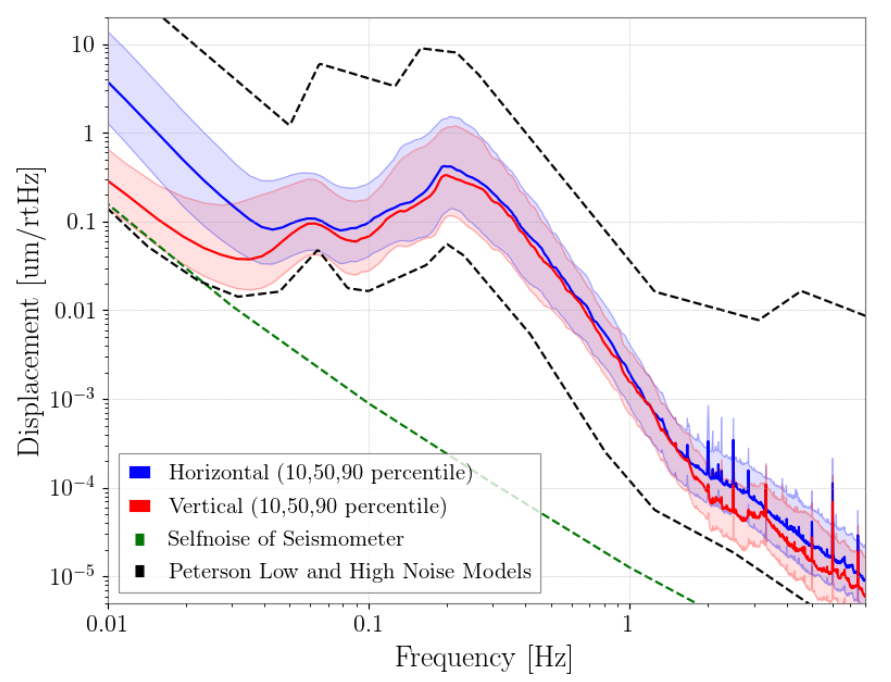
\includegraphics[width=13.0cm]{./img_chap3/img313.png}
    \caption{}\label{img:img313}
  \end{center}
\end{figure}


%\newpage
\section{Study of Differential Motion Reduction}\label{sec:34}
\subsection{Introduction}
The motion of two mirrors in the cavity have two modes. One is differential motion, which is the length change of that. Another one is common motion, which is the motion of the center of the cavity. In terms of the length control, it is important that the RMS amplitude of differential motion is as small as possible. Actuarlly, the amplitude of these two motions are the same each other when the mirrors moves with no coherence. However, when a coherence exists, the common motion tends to be larger than the differential one. 

As discussed in this section, the coherence depends on both, the arm length and the wavelength of seismic waves. For example, if the arm length is much more smaller than the wavelength, the mirrors move together. This means that the common motion is greater than the differential motion.

The ratio of the amplitudes of the differential motion over common motion is newly defined as Common and Differential Motion Ratio (CDMR). It is usefull to know how the ground reducts the differential motion or increase the common motion. 

\subsection{Overview}
Fig.\ref{img:img318}に示すように

\begin{figure}[H]
  \begin{center}   
    
\includegraphics[width=10.0cm]{./img_chap3/img318.png}
    \caption{Seismometers for measurement of the differential motion redction}\label{img:img318}
  \end{center}
\end{figure}


\subsection{Reduction in X-arm Scale}



\subsection{Reduction in Other Short Scale}

\begin{figure}[p]
  \begin{minipage}{0.65\hsize}  
    \begin{center}   
      
\includegraphics[width=10.0cm]{./img_chap3/img319.png}
      \caption{...}\label{img:img319}
    \end{center}
  \end{minipage}
  \begin{minipage}{0.65\hsize}  
    \begin{center}   
      
\includegraphics[width=10.0cm]{./img_chap3/img320.png}
      \caption{...}\label{img:img320}
    \end{center}
  \end{minipage}    
\end{figure}



\section{Summary of the Chapter}
